\chapter{Sensor Application}\label{sensor-application}
In this chapter a sensor application will be presented. 
Several sequence diagrams will be explained, as well as concepts needed to understand the flow of the application. 

\section{Physical Connection Initialization}\label{physical_connection_initialization}
One of the best solutions for authentication of an identity in cryptography is rendezvous authentication, the concept of meeting face-to-face for athentication. 
In \gls{IoT}, we have in most cases the advantage of identifying devices in a physical matter. 
This means that it is possible to authenticate devices, such as sensors. 
Typically, this kind of authentication will rely on 1) manually inspection and 2) digital connection, e.g. through \gls{NFC}.

\section{Health Sensors}
Hacking insulin pump~\cite{radcliffe2011hacking}

\section{Application}


\subsection{Initialization}
~\autoref{fig:init_ibe_2}

\begin{enumerate}
  \item First device, e.g. a mobile, connects to the \gls{PKG} through physical connection (discussed in~\autoref{physical_connection_initialization}) as showed in~\autoref{fig:init_ibe_1}.
  \item Additional devices can connect through physical connection (discussed in~\autoref{physical_connection_initialization}) via another authorized device~\autoref{fig:init_ibe_2}, or the \gls{PKG} itself~\autoref{fig:init_ibe_1}. 
  \item Data pulling from existing nodes in network~\autoref{fig:data_pull_ibe}
\end{enumerate}

\begin{figure}[ht]
  \centering
  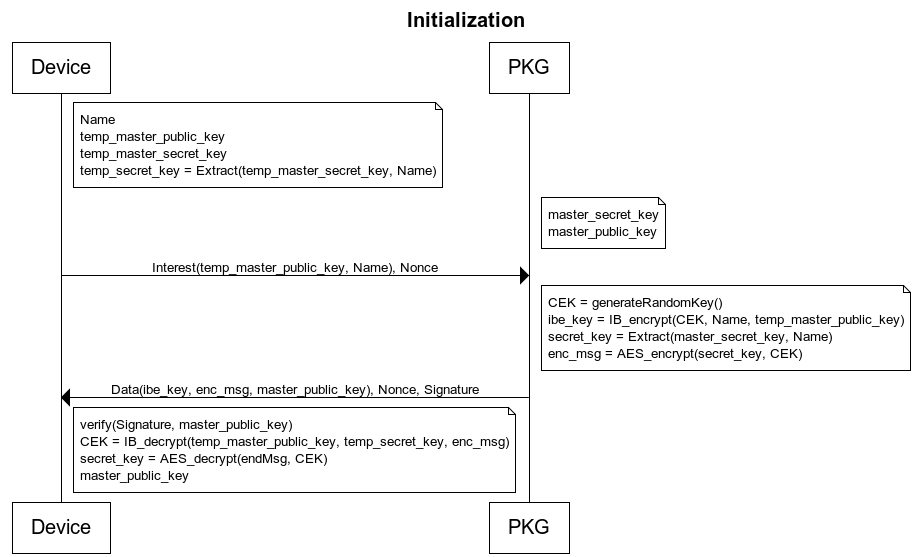
\includegraphics[width=1\textwidth]{Initialization.png}
  \caption{Initialization IBE}
  \label{fig:init_ibe_1}
\end{figure}

Every device should connect to mobile thorugh e.g. \gls{NFC} for initialization.
This results in a physical authentication between the device, and the mobile (i.e. the end user).

\begin{figure}[ht]
  \centering
  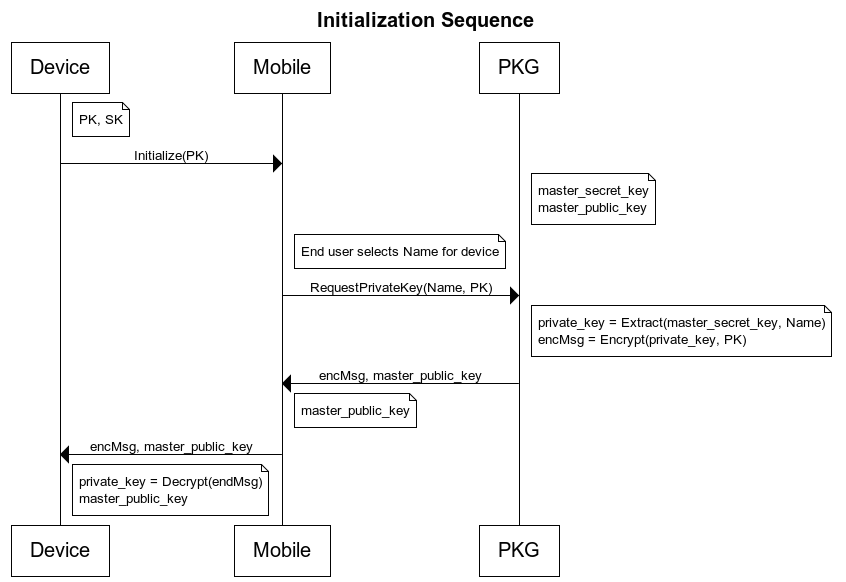
\includegraphics[width=1\textwidth]{init_ibe_2.png}
  \caption{Initialization IBE through authorized device}
  \label{fig:init_ibe_2}
\end{figure}

% \begin{lstlisting}[language=BASH, caption={Initialization}, label={lst:ibe-initialization}]
% pkg = new PublicKeyGenerator;
% for device in {devices}
% do
% 	device -> connect to pkg;
% 	pkg -> verify device then issue Private Key;
% 	device -> subscribe Name Sync and Public Key
% done
% \end{lstlisting}


\subsection{Identity-Based Cryptography}

\section{Integrity and Authenticity}

Each device will obtain a private key allocated by its superior \gls{PKG}, as explained in~\autoref{ibc}.
With the concept from~\autoref{physical_connection_initialization} together with the \gls{PKG}s \gls{MPK}, you can trust that the device is authorized for the \gls{PKG}s network. Hence all signed packets can be verified by anyone with the \gls{MPK}.

\subsection{Replay Attack}
Every Interest has a timestamp attached to the Name (e.g. /ndn/no/ntnu/device/name2/sensor\_pull/\textbf{1429710873778}), i.e. milliseconds from UTC 1970-01-01 00:00:00, that is used for protection against replay attack. 

\section{Confidentiality}

All data can be, if needed, encrypted.
The encryption can be achieved by encrypting with the Name of the requester as the public key.


\section{Availability}

This is a harder problem to solve.
The network is purely wireless, hence vulnerable to jamming. 

\subsection{Access Control}

When a device retrieves an Interest for its sensor data, there should be a authorization mechanism. 
In~\autoref{fig:data_pull_ibe} 
\begin{figure}[ht]
  \centering
  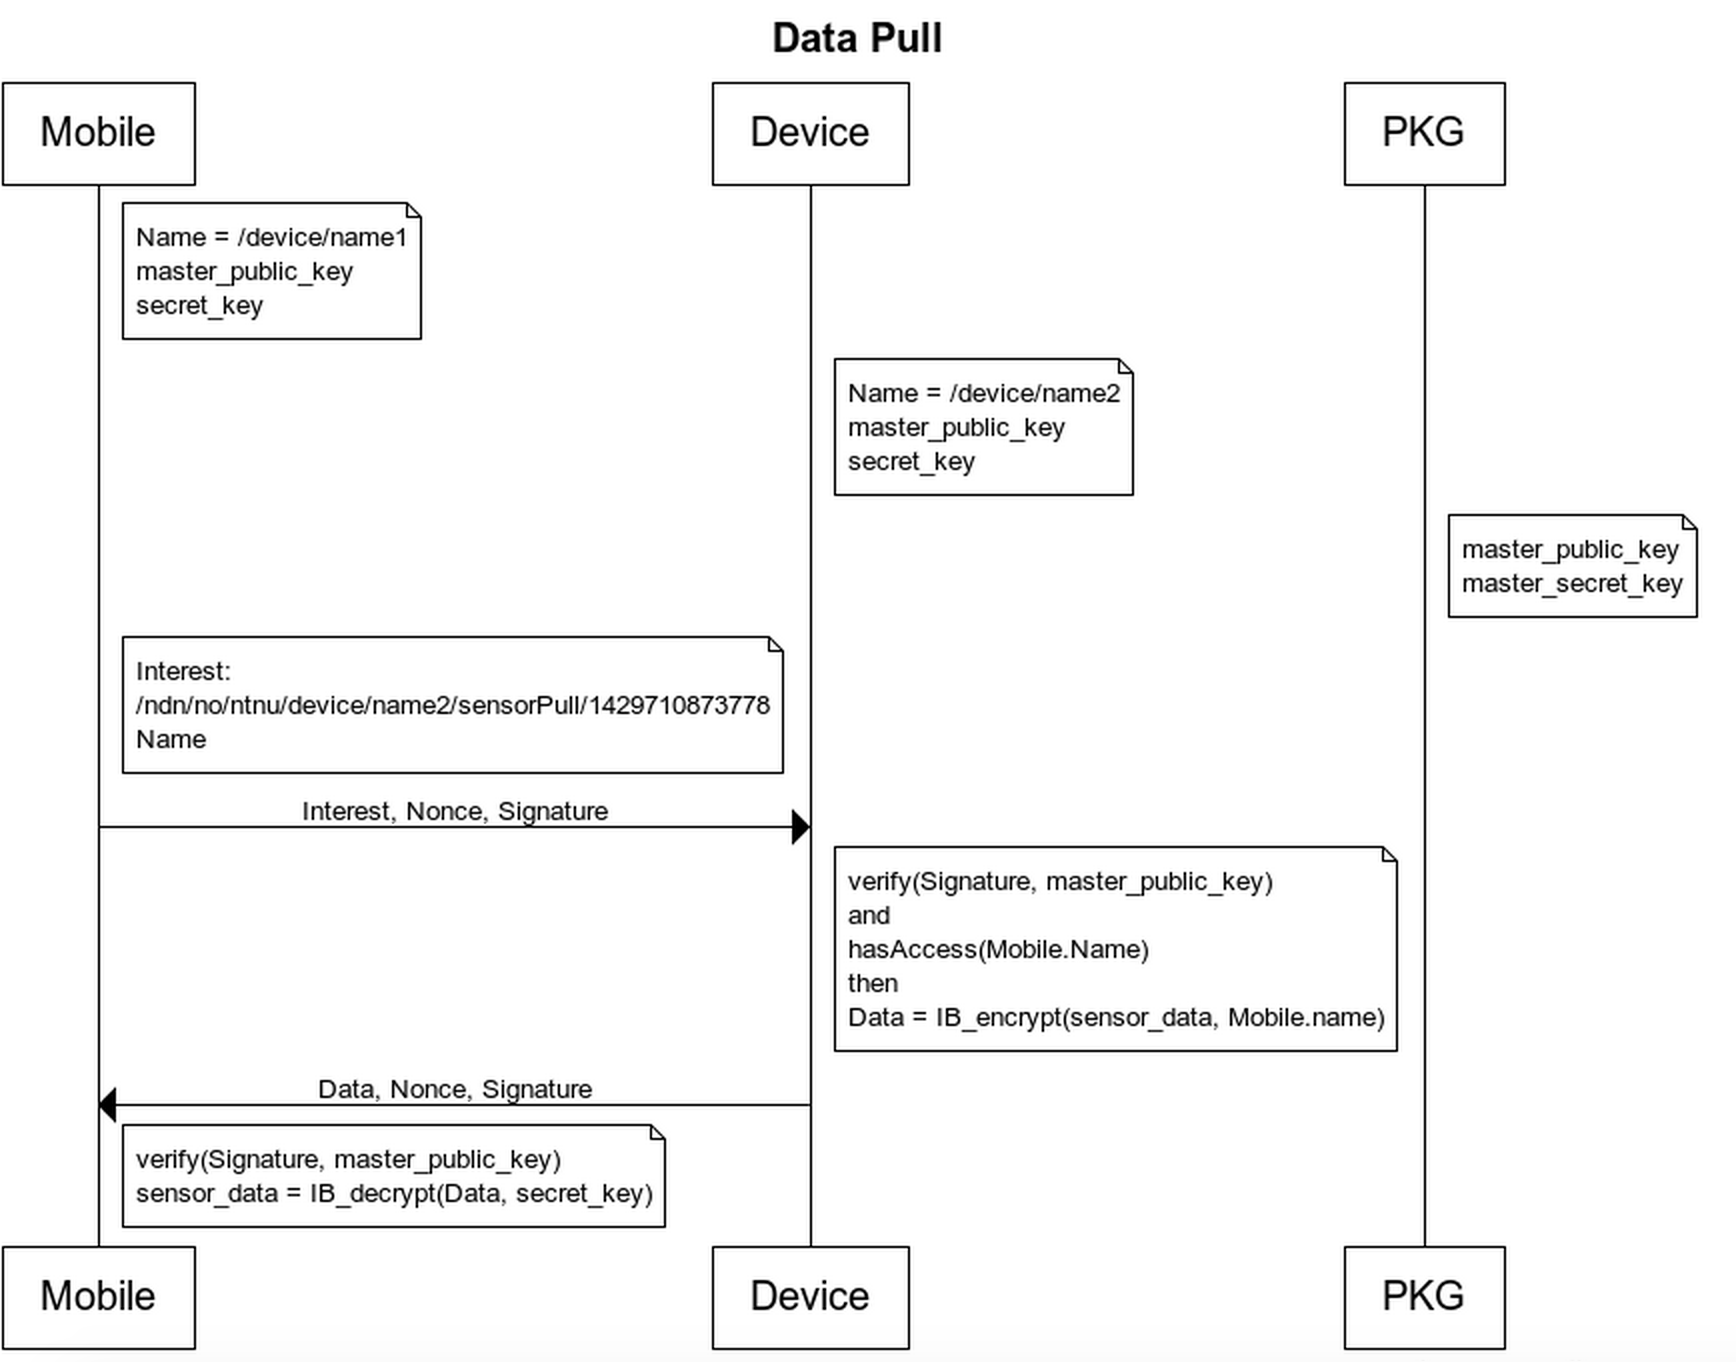
\includegraphics[width=1\textwidth]{DataPull.png}
  \caption{Mobile performing a data pull from a device in the network.}
  \label{fig:data_pull_ibe}
\end{figure}


Capability based approach to \gls{IoT} access control~\cite{DBLP:conf/imis/GusmeroliPR12}.

Least privilege access